\section{Dataset and Preprocessing}
\label{sec:Data Analysis and Preparation}


% \subsection{Dataset Details}
% The dataset used in this study is characterised by the following properties.
% \begin{description}
%   \item[Source:] DCASE~2020 Task~2 Development—slide-rail class
%   \item[Size:] $\approx$3 machine IDs
%   \item[Duration per file:] $\sim$10 s mono\;@\;16 kHz
%   \item[Environment:] Real-world factory background noise
% \end{description}
% The data set used for this project consists of 3471 WAV format sound files labelled either as normal or as anomalies, and divided into a development set of 2370 files with only normal labelled files, and a test set of 1101 files which is made of both classes, 300 normal and 801 anomalies. For monitoring the model's performance across epochs, the development set is divided into a training and a validation set using a 90-10 split.

% The labels are inferred from the filenames, which follow the format \textit{normal/anomaly\_id\_id-number\_sample-number.wav}. For example, \textit{anomaly\_id\_00\_00000015.wav} indicates an anomalous sample. 

% ---------- Subsection: Dataset Details ----------
\subsection{Dataset Details}
\vspace{0.2em}
\noindent
\textbf{Source.}  
All recordings originate from the \emph{MIMII} slide–rail subset introduced by Purohit
\textit{et~al.}\ \cite{purohit2019mimii}.  
This subset constitutes one of the machine types distributed as
development data for \textbf{DCASE 2020 Task 2} on unsupervised anomalous–sound
detection in machine condition monitoring.

\noindent
\textbf{Machine IDs and split.}
The corpus contains \emph{exactly three} machine identities (ID~00, 02, 04).
For each ID, only normal recordings are provided for training
(``dev\_train''), whereas both normal and anomalous examples appear in the
evaluation (``dev\_test'') set:

\begin{table}[h]
\centering
\begin{tabular}{lccc}
\toprule
\textbf{ID} & \textbf{Normal (train)} & \textbf{Normal / Anom.\ (test)} & \textbf{Duration} \\
\midrule
00 & 790 & 100 / 356 & 10 s \\
02 & 790 & 100 / 267 & 10 s \\
04 & 790 & 100 / 178 & 10 s \\
\midrule
\textbf{Total} & 2370 & 300 / 801 & \\
\bottomrule
\end{tabular}
\caption{File counts per machine ID (16 kHz mono).}
\label{tab:id_split}
\end{table}

\noindent
\textbf{Recording conditions.}  
Audio was captured with microphones mounted inside a real factory
environment and therefore includes non-stationary background noise.
Each file is ten seconds long, single-channel, and stored as 16-bit
\texttt{.wav} at 16\,kHz.

\noindent
\textbf{File-name convention.}  
Labels are inferred from the canonical naming scheme
\texttt{\{normal$\vert$anomaly\}\_id\_\{ID\}\_\{NNNNNNNN\}.wav}; e.g.,
\texttt{anomaly\_id\_00\_00000015.wav} designates an anomalous
recording of machine ID~00.

\noindent
\textbf{Usage in this work.}  
We adopt the official split: \emph{dev\_train} (normal-only) for model
training, a 10\,\% held-out slice of the same set for parameter
selection, and \emph{dev\_test} for final reporting.  This mirrors the
zero-positive learning scenario mandated by Task 2.


\subsection{Feature Extraction}
The complete preprocessing pipeline is summarised below:

\begin{enumerate}
  \item \textbf{Short-time Fourier transform (STFT)} with a 1024-sample Hann window and a 512-sample hop (approximately 64~ms and 32~ms, respectively) to expose local spectral content.
  \item \textbf{Mel filterbank} with 64 triangular bands spanning 0–8~kHz, reflecting the frequency resolution of human hearing.
  \item \textbf{Logarithmic compression} using the formula \( \log(1 + 10 \times |\mathrm{Mel}|) \) for variance stabilisation and dynamic-range reduction.
  \item \textbf{Per-file min–max normalisation} to the range \([0, 1]\), followed by \textbf{global standardisation} (zero mean, unit variance) based on training statistics.
\end{enumerate}

% Approaching the intended task in the 1D-domain of the provided raw audio signals diminishes anomaly detection capabilities, as this representation does not expose frequency content, which is key for this task as anomalies are often frequency-localized. Instead, to expose this frequency based patterns as well as reducing data complexity and focusing on relevant structure, this raw signals are transformed into spectrograms, specifically to Log-Mel ones, which compose a more aligned representation with human perception. The resulting are normalized to zero mean and unit variance to improve training stability and help the model focus on scale-invariant features, as preserving relative amplitudes is more important than retaining absolute amplitudes.

Raw audio waveforms are first down-sampled to 16~kHz and transformed into time–frequency representations to better expose spectral regularities where anomalies typically manifest.  
Approaching the task directly in the time domain diminishes anomaly detection capability, as raw waveforms do not reveal frequency-localised patterns that are key indicators of malfunctioning behavior.

To obtain a perceptually meaningful and compact representation, we compute 64-band log-Mel spectrograms. A 1024-sample Hann window (\(\approx\)64~ms) with a 512-sample hop (\(\approx\)32~ms) is applied to perform the short-time Fourier transform (STFT).  
This configuration balances temporal acuity and frequency resolution—sufficient, for example, to capture the $\sim$300~ms mechanical cycle of a typical slide operation.

The Mel spectrogram is then compressed using a log transformation to stabilise variance and reduce dynamic range:
\[
X_{d,b} = \log\left(1 + 10 \cdot M_{d,b}\right),
\]
where \( M_{d,b} \) denotes the Mel energy for frame \( d \) and frequency band \( b \).  
Subsequently, each spectrogram is min–max normalised per file, followed by global standardisation using statistics computed from the training set.  
This ensures that gain variations across sessions do not bias the anomaly score, while allowing the model to focus on scale-invariant structure rather than absolute amplitudes.
Figure \ref{fig:LogMel Viz} visualises two normal and two anomalous examples from the two different machines (ID-00 and ID-02):

\begin{figure}
    \centering
    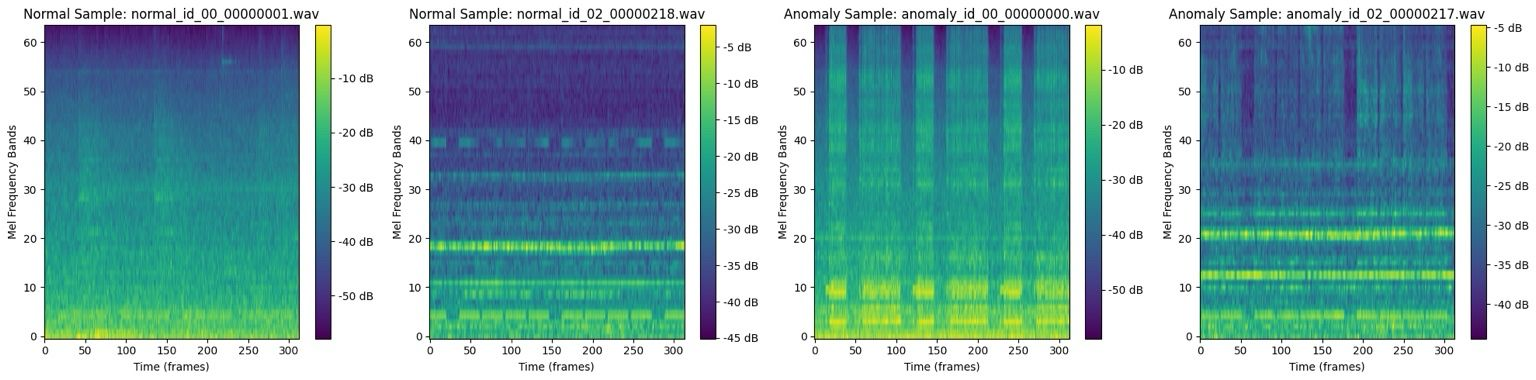
\includegraphics[width=1\linewidth]{Figures/logmel viz.jpeg}
    \caption{Visualization of Mel Spectogram on Normal and Anomaly Machines}
    \label{fig:LogMel Viz}
\end{figure}

% 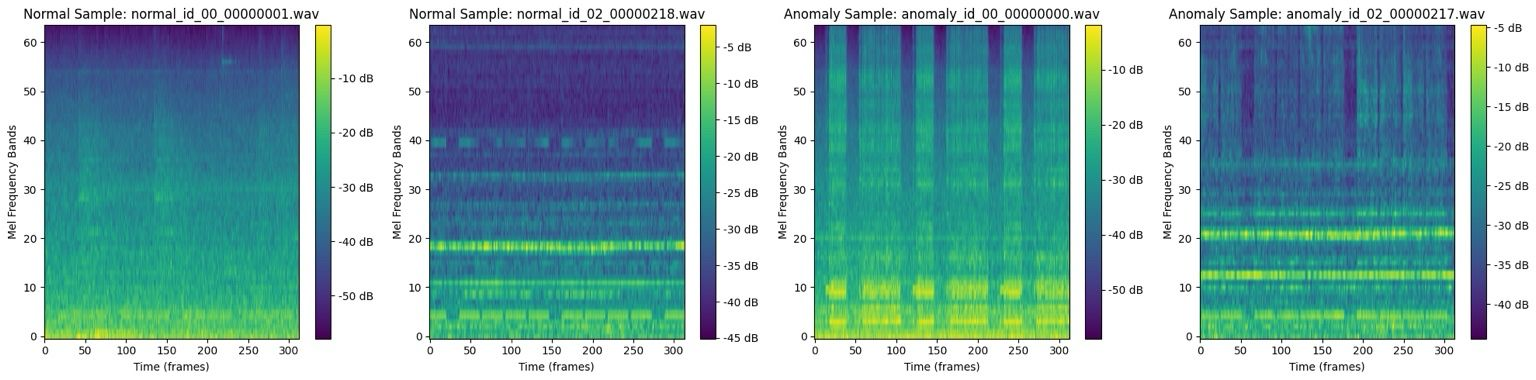
\includegraphics[width=1\textwidth]{Figures/logmel viz.jpeg}
% \label{fig:LogMel Viz}

Figure~\ref{fig:LogMel Viz} shows that anomalous samples notably lack the low-frequency ridges characteristic of healthy operation and exhibit pronounced \emph{vertical stripes} that signal abnormal friction.












